\documentclass[portrait, slides]{seminar}

\usepackage{semcolor} % For coloured text.
\usepackage{slidesec} % For section headings.
\usepackage{newcent}  % This is a better font for presentations.
\input{seminar.bug}

\usepackage{graphicx} % For pictures.
\usepackage{fancybox} % For the background picture.

\renewcommand{\slidetopmargin}{-2cm} % Actually the left margin (landscape).
\addtolength{\slidewidth}{1cm}       % Otherwise the text doesn't look good.
\renewcommand{\sliderightmargin}{-1cm}
%\addtolength{\slideheight}{3cm}

\newslideframe{IMAGE}{ % The picture bg.eps is a picture in a4 format.
  \boxput{
    \rput(-.81, -1.21){
\includegraphics[angle=90, scale=.485]{bg}}
    \rput[l]{90}(-3.7, -8.36){
\includegraphics[scale=.03]{bullet0} 
                                \white $_\mathrm{\bf{Introduction}}$}
    \rput[l]{90}(-3.3, -8.36){
\includegraphics[scale=.03]{bullet0} 
                                \white $_\mathrm{\bf{Rauzy}}$}
    \rput[l]{90}(-2.9, -8.36){
\includegraphics[scale=.03]{bullet0} 
                                \white $_\mathrm{\bf{DNA}}$}
    \rput[l]{90}(-2.5, -8.36){
\includegraphics[scale=.03]{bullet0} 
                                \white $_\mathrm{\bf{Hyperplanes}}$}
    \rput[l]{90}(-2.1, -8.36){
\includegraphics[scale=.03]{bullet0} 
                                \white $_\mathrm{\bf{Results}}$}
    \rput[l]{90}(-1.7, -8.36){
\includegraphics[scale=.03]{bullet0} 
                                \white $_\mathrm{\bf{Conclusions}}$}
    \rput[l]{90}(-1.3, -8.36){
\includegraphics[scale=.03]{bullet0} 
                                \white $_\mathrm{\bf{Questions?}}$}
%    \rput[l]{90}(-0.9, -8.36){
\includegraphics[scale=.03]{bullet0} 
%                                \white $_\mathrm{\bf{Item 7}}$}
%    \rput[l]{90}(-0.5, -8.36){
\includegraphics[scale=.03]{bullet0} 
%                                \white $_\mathrm{\bf{Conclusions}}$}
%    \rput[l]{90}(-0.1, -8.36){
\includegraphics[scale=.03]{bullet0} 
%                                \white $_\mathrm{\bf{Questions?}}$}
  }{#1}}
\slideframe{IMAGE}

\pagestyle{empty}

\begin{document}

\begin{slide}
\rput[l](-2.936, -0.21){
\includegraphics[scale=.03]{bullet1}}

\begin{center}
\Huge{Visualising DNA with Rauzy Projections}\\
\vspace{1cm}
\small{Hendrik Jan Hoogeboom$^1$, Walter A. Kosters$^1$, 
       {\bf Jeroen F. J. Laros}$^1$\\
       and Sjoerd M. Verduyn Lunel$^2$}\\
\small{$^1$ Leiden Institute of Advanced Computer Science}\\
\small{$^2$ Mathematical Institute}\\
\small{Leiden University}
\end{center}
\vfill
\end{slide}

\begin{slide}
\rput[l](-2.936, -0.21){
\includegraphics[scale=.03]{bullet1}}

\slideheading{Pattern recognition}
\begin{center}
$\mathtt{ababababababababababababababababababababababa}\ldots$\\
$(\mathtt{ab})^*$\\
\vspace{2ex}
$\mathtt{abbbababaaababbabbbababaaababbabbbababaaababb}\ldots$\\
$(\mathtt{abbbababaaababb})^*$\\
\vspace{2ex}
$\mathtt{abaaaababbbbabaaaababbbbabaaaababbbbabaaaabab}\ldots$\\
$(\mathtt{abaaaa}\cdot\mathtt{babbbb})^*$
\vspace{2ex}
\end{center}
Long patterns over small alphabets can become very hard to find, especially
when small deviations are allowed.
\vfill
\end{slide}

\begin{slide}
\rput[l](-2.936, -0.21){
\includegraphics[scale=.03]{bullet1}}
%\rput[l](-2.936, -0.98){
\includegraphics[scale=.03]{bullet1}}
%\rput[l](-2.936, -1.38){
\includegraphics[scale=.03]{bullet1}}
%\rput[l](-2.936, -1.81){
\includegraphics[scale=.03]{bullet1}}
%\rput[l](-2.936, -2.185){
\includegraphics[scale=.03]{bullet1}}
%\rput[l](-2.936, -2.585){
\includegraphics[scale=.03]{bullet1}}
%\rput[l](-2.936, -2.98){
\includegraphics[scale=.03]{bullet1}}
%\rput[l](-2.936, -3.405){
\includegraphics[scale=.03]{bullet1}}

\slideheading{Pattern visualisation example}
\scalebox{.4}{
\input{ab.pstex} \input{abbbababaaababb.pstex}
}
\begin{picture}(0,0)(285,85)
\thicklines
\put(0,0){\vector(1,0){30}}
\put(12,-7){$\mathtt{a}$}
\put(0,0){\vector(0,1){30}}
\put(-7,12){$\mathtt{b}$}
%\put(0,0){\vector(1,1){15}}
%\put(4,10){$\mathtt{c}$}
\end{picture}
\begin{center}
\scalebox{.4}{
\input{abaaaa.pstex}
}
\end{center}

\vfill
\end{slide}

\begin{slide}
\rput[l](-2.936, -0.61){
\includegraphics[scale=.03]{bullet1}}
%\rput[l](-2.936, -0.98){
\includegraphics[scale=.03]{bullet1}}
%\rput[l](-2.936, -1.38){
\includegraphics[scale=.03]{bullet1}}
%\rput[l](-2.936, -1.81){
\includegraphics[scale=.03]{bullet1}}
%\rput[l](-2.936, -2.185){
\includegraphics[scale=.03]{bullet1}}
%\rput[l](-2.936, -2.585){
\includegraphics[scale=.03]{bullet1}}
%\rput[l](-2.936, -2.98){
\includegraphics[scale=.03]{bullet1}}
%\rput[l](-2.936, -3.405){
\includegraphics[scale=.03]{bullet1}}

\slideheading{Rauzy fractals}
\begin{itemize}
\item A \red Rauzy Fractal \black is a two dimensional projection of a three
      dimensional spacial structure.
\item The three dimensional spacial structure is strongly related to the 
      fixed point of a $\beta$-substitution (e.g., the Tribonacci substitution,
      see later).
\item The structure is projected on the plane that is ``most'' perpendicular
      to the structure.
\item The typical Rauzy fractal has three colours. The colour of each point
      is determined by the next direction in the spacial structure.
\end{itemize}

\vfill
\end{slide}

\begin{slide}
\rput[l](-2.936, -0.61){
\includegraphics[scale=.03]{bullet1}}
%\rput[l](-2.936, -0.98){
\includegraphics[scale=.03]{bullet1}}
%\rput[l](-2.936, -1.38){
\includegraphics[scale=.03]{bullet1}}
%\rput[l](-2.936, -1.81){
\includegraphics[scale=.03]{bullet1}}
%\rput[l](-2.936, -2.185){
\includegraphics[scale=.03]{bullet1}}
%\rput[l](-2.936, -2.585){
\includegraphics[scale=.03]{bullet1}}
%\rput[l](-2.936, -2.98){
\includegraphics[scale=.03]{bullet1}}
%\rput[l](-2.936, -3.405){
\includegraphics[scale=.03]{bullet1}}

\slideheading{Classical Rauzy fractal}
Let $\{0, 1, 2\}$ be an alphabet. 

The Tribonacci substitution is as follows:
\[
\sigma: \left\{
\begin{array}{lll}
0 & \rightarrow & 01\\
1 & \rightarrow & 02\\
2 & \rightarrow & 0
\end{array}
\right.
\]

There is one (infinite) word invariant under this substitution; its 
\red fixed point\black:\\

\begin{center}
$\mathtt{010201001020101020100102010201001020101020100}\ldots$
\end{center}

\vfill
\end{slide}

\begin{slide}
\rput[l](-2.936, -0.61){
\includegraphics[scale=.03]{bullet1}}
%\rput[l](-2.936, -0.98){
\includegraphics[scale=.03]{bullet1}}
%\rput[l](-2.936, -1.38){
\includegraphics[scale=.03]{bullet1}}
%\rput[l](-2.936, -1.81){
\includegraphics[scale=.03]{bullet1}}
%\rput[l](-2.936, -2.185){
\includegraphics[scale=.03]{bullet1}}
%\rput[l](-2.936, -2.585){
\includegraphics[scale=.03]{bullet1}}
%\rput[l](-2.936, -2.98){
\includegraphics[scale=.03]{bullet1}}
%\rput[l](-2.936, -3.405){
\includegraphics[scale=.03]{bullet1}}

\slideheading{Rauzy's spacial pattern}
\scalebox{.4}{
\input{trib.pstex} \input{trib2.pstex}
}
\begin{picture}(0,0)(275,80)
\thicklines
\put(0,0){\vector(1,0){30}}
\put(12,-7){$\mathtt{0}$}
\put(0,0){\vector(0,1){30}}
\put(-7,12){$\mathtt{2}$}
\put(0,0){\vector(1,1){15}}
\put(4,10){$\mathtt{1}$}
\end{picture}
\begin{center}
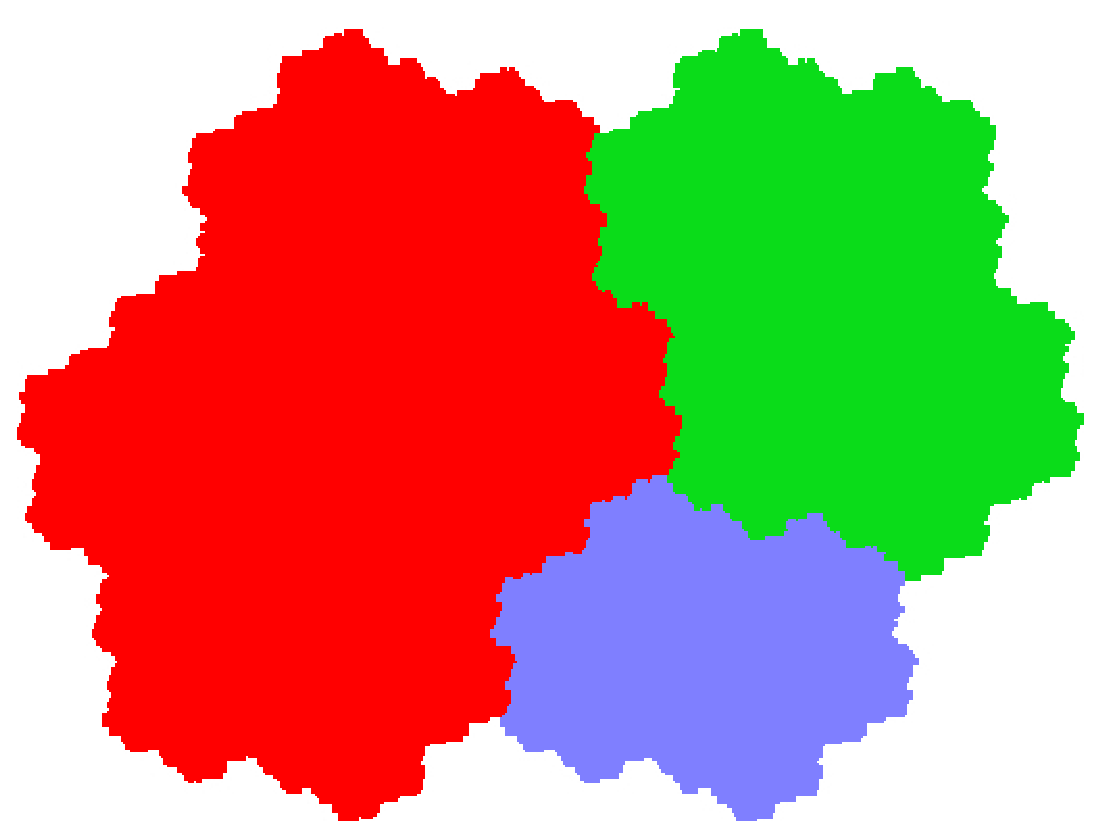
\includegraphics[scale=.2]{017}
\end{center}

\vfill
\end{slide}

\begin{slide}
\rput[l](-2.936, -0.61){
\includegraphics[scale=.03]{bullet1}}
%\rput[l](-2.936, -0.98){
\includegraphics[scale=.03]{bullet1}}
%\rput[l](-2.936, -1.38){
\includegraphics[scale=.03]{bullet1}}
%\rput[l](-2.936, -1.81){
\includegraphics[scale=.03]{bullet1}}
%\rput[l](-2.936, -2.185){\includegraphics[scale=.03]{bullet1}}
%\rput[l](-2.936, -2.585){\includegraphics[scale=.03]{bullet1}}
%\rput[l](-2.936, -2.98){\includegraphics[scale=.03]{bullet1}}
%\rput[l](-2.936, -3.405){\includegraphics[scale=.03]{bullet1}}

\slideheading{Other ``Rauzy'' fractals}
The substitution:
\[
\sigma: \left\{
\begin{array}{lll}
0 & \rightarrow & 01\\
1 & \rightarrow & 2\\
2 & \rightarrow & 0
\end{array}
\right.
\]
results in the following fractal by using the same construction:

\begin{center}
\includegraphics[scale=.2]{006}
\end{center}

\vfill
\end{slide}

\begin{slide}
\rput[l](-2.936, -0.98){\includegraphics[scale=.03]{bullet1}}
%\rput[l](-2.936, -1.38){\includegraphics[scale=.03]{bullet1}}
%\rput[l](-2.936, -1.81){\includegraphics[scale=.03]{bullet1}}
%\rput[l](-2.936, -2.185){\includegraphics[scale=.03]{bullet1}}
%\rput[l](-2.936, -2.585){\includegraphics[scale=.03]{bullet1}}
%\rput[l](-2.936, -2.98){\includegraphics[scale=.03]{bullet1}}
%\rput[l](-2.936, -3.405){\includegraphics[scale=.03]{bullet1}}

\slideheading{Using naturally occurring strings}
We can apply a similar technique using strings from nature: 

\begin{itemize}
\item Associate each nucleotide with a spacial dimension (we need four
      dimensions now).
\item Build a spacial structure analogous to the construction of the Rauzy
      fractal.
\item \red Choose \black a plane or hyperplane for the projection.
\end{itemize}

Since a DNA string is finite and does not have the nice mathematical properties
that the Tribonacci fixed point has, there is no clear preference for a line
along which we can project the structure. In other words, the ``most''
perpendicular (hyper)plane is dependent on the input.

\vfill
\end{slide}

\begin{slide}
\rput[l](-2.936, -0.98){\includegraphics[scale=.03]{bullet1}}
%\rput[l](-2.936, -1.38){\includegraphics[scale=.03]{bullet1}}
%\rput[l](-2.936, -1.81){\includegraphics[scale=.03]{bullet1}}
%\rput[l](-2.936, -2.185){\includegraphics[scale=.03]{bullet1}}
%\rput[l](-2.936, -2.585){\includegraphics[scale=.03]{bullet1}}
%\rput[l](-2.936, -2.98){\includegraphics[scale=.03]{bullet1}}
%\rput[l](-2.936, -3.405){\includegraphics[scale=.03]{bullet1}}

\slideheading{Hypotheses}
When the (hyper)plane is chosen well, we expect to see the following things
in the projected image:
\vspace{1cm}
\begin{itemize}
\item A non-predictable walk for information rich parts of the DNA.
\item A true random walk for random parts.
\item Lines (or approximate lines) for repeating parts of the DNA.
\item Large copies of substrings in the DNA, that can be easily visualised.
\end{itemize}

\vfill
\end{slide}

\begin{slide}
%\rput[l](-2.936, -0.98){\includegraphics[scale=.03]{bullet1}}
\rput[l](-2.936, -1.38){\includegraphics[scale=.03]{bullet1}}
%\rput[l](-2.936, -1.81){\includegraphics[scale=.03]{bullet1}}
%\rput[l](-2.936, -2.185){\includegraphics[scale=.03]{bullet1}}
%\rput[l](-2.936, -2.585){\includegraphics[scale=.03]{bullet1}}
%\rput[l](-2.936, -2.98){\includegraphics[scale=.03]{bullet1}}
%\rput[l](-2.936, -3.405){\includegraphics[scale=.03]{bullet1}}

\slideheading{How to choose the (hyper)plane}
We can translate the choice of the (hyper)plane to the choice of four vectors
in the resulting projection, in this case, four three-dimensional vectors.

In order to get an insightful projection, we want the vectors to have the 
following properties:
\vspace{.5cm}
\begin{itemize}
\item The vectors should be of comparable length.
\item The \red four \black vectors should add up to 0.
\item Every subset of three vectors should be independent.
\end{itemize}

\vfill
\end{slide}

\begin{slide}
\rput[l](-2.936, -1.38){\includegraphics[scale=.03]{bullet1}}
%\rput[l](-2.936, -1.38){\includegraphics[scale=.03]{bullet1}}
%\rput[l](-2.936, -1.81){\includegraphics[scale=.03]{bullet1}}
%\rput[l](-2.936, -2.185){\includegraphics[scale=.03]{bullet1}}
%\rput[l](-2.936, -2.585){\includegraphics[scale=.03]{bullet1}}
%\rput[l](-2.936, -2.98){\includegraphics[scale=.03]{bullet1}}
%\rput[l](-2.936, -3.405){\includegraphics[scale=.03]{bullet1}}

\slideheading{Our choice for the three dimensional hyperplane}
We use the set of vectors that defines a tetrahedron (centred at the origin):

\[
\left(
\begin{array}{rrrr}
1 & -1 & -1 &  1\\
1 & -1 &  1 & -1\\
1 &  1 & -1 & -1\\
\end{array}
\right)
\]

\vspace{0.5cm}
All vectors are of \red equal \black length and they are \red uniformly 
distributed\black, the angle between each pair of vectors is equal.

\vfill
\end{slide}

\begin{slide}
\rput[l](-2.936, -1.81){\includegraphics[scale=.03]{bullet1}}
%\rput[l](-2.936, -2.185){\includegraphics[scale=.03]{bullet1}}
%\rput[l](-2.936, -2.585){\includegraphics[scale=.03]{bullet1}}
%\rput[l](-2.936, -2.98){\includegraphics[scale=.03]{bullet1}}
%\rput[l](-2.936, -3.405){\includegraphics[scale=.03]{bullet1}}

\slideheading{3D results}
\vspace{-0.5cm}
\begin{center}
\includegraphics[angle=270, scale=.2]{y-3d} \includegraphics[angle=270, scale=.2]{y2-3d}

The first $160,\!000$ nucleotides of the human Y-chromosome.
\end{center}

\vspace{0.5cm}
The input data is the same, different angles are used to view the data.

\vfill
\end{slide}

\begin{slide}
\rput[l](-2.936, -1.81){\includegraphics[scale=.03]{bullet1}}
%\rput[l](-2.936, -0.98){\includegraphics[scale=.03]{bullet1}}
%\rput[l](-2.936, -1.38){\includegraphics[scale=.03]{bullet1}}
%\rput[l](-2.936, -1.81){\includegraphics[scale=.03]{bullet1}}
%\rput[l](-2.936, -2.185){\includegraphics[scale=.03]{bullet1}}
%\rput[l](-2.936, -2.585){\includegraphics[scale=.03]{bullet1}}
%\rput[l](-2.936, -2.98){\includegraphics[scale=.03]{bullet1}}
%\rput[l](-2.936, -3.405){\includegraphics[scale=.03]{bullet1}}

\slideheading{3D results}
\begin{center}
\vspace{-2cm}
\includegraphics[angle=270, scale=.35]{1-3d}

Offset $40,\!000$--$100,\!000$ of the human chromosome 1. 
\end{center}
\vfill
\end{slide}

\begin{slide}
\rput[l](-2.936, -1.81){\includegraphics[scale=.03]{bullet1}}
%\rput[l](-2.936, -0.98){\includegraphics[scale=.03]{bullet1}}
%\rput[l](-2.936, -1.38){\includegraphics[scale=.03]{bullet1}}
%\rput[l](-2.936, -1.81){\includegraphics[scale=.03]{bullet1}}
%\rput[l](-2.936, -2.185){\includegraphics[scale=.03]{bullet1}}
%\rput[l](-2.936, -2.585){\includegraphics[scale=.03]{bullet1}}
%\rput[l](-2.936, -2.98){\includegraphics[scale=.03]{bullet1}}
%\rput[l](-2.936, -3.405){\includegraphics[scale=.03]{bullet1}}

\slideheading{A selected 2D projection}
\begin{center}
\includegraphics[angle=270, scale=.3]{160000}

The first $160,\!000$ nucleotides of the human Y-chromosome.
\end{center}

\vfill
\end{slide}

\begin{slide}
%\rput[l](-2.936, -0.98){\includegraphics[scale=.03]{bullet1}}
%\rput[l](-2.936, -1.38){\includegraphics[scale=.03]{bullet1}}
%\rput[l](-2.936, -1.81){\includegraphics[scale=.03]{bullet1}}
\rput[l](-2.936, -2.185){\includegraphics[scale=.03]{bullet1}}
%\rput[l](-2.936, -2.585){\includegraphics[scale=.03]{bullet1}}
%\rput[l](-2.936, -2.98){\includegraphics[scale=.03]{bullet1}}
%\rput[l](-2.936, -3.405){\includegraphics[scale=.03]{bullet1}}

\slideheading{Conclusions}
\vspace{1cm}
\begin{itemize}
\item Simple repeats can easily be detected.
\item Large repeats can also easily be seen.
\item Extremely large approximate repeats can be seen.
\item No excessive calculation has to be done in order to find these 
      properties.
\end{itemize}

\vspace{.5cm}
See \small{\texttt{http://www.liacs.nl/home/jlaros/projects/dnavis/}} for an
interactive demo.

\vfill
\end{slide}

\begin{slide}
%\rput[l](-2.936, -3.780){\includegraphics[scale=.03]{bullet1}}
\rput[l](-2.936, -2.585){\includegraphics[scale=.03]{bullet1}}
\slideheading{Questions?}
\vspace*{4cm}
\tiny{
This research is part of the DALE (Data Assistance for Law Enforcement)
project as financed in the ToKeN program from the Netherlands Organization
for Scientific Research (NWO) under grant number 634.000.430.
}
\begin{center}
\begin{figure}
\vspace{0.7cm}
\includegraphics[scale=0.085]{nwo}
\hspace{4cm}
\includegraphics[scale=0.15]{token}
\end{figure}
\end{center}
\vfill
\end{slide}

\end{document}
